V tejto kapitole, uvedieme niektoré zo štatistýk týkajúcich sa generovania herných svetov, zanalyzujeme ich a úkážeme si vygenerovaný príbeh našou aplikáciou.
\section{Štatistiky generovania svetov}
Pri rozhodovaní koľko náhodných herných svetov naraz je vhodné generovať, sme museli počitať s tým, aby boli vyvážené hodnoty času generovania a dostatočného ohodnotenia príbehu. Nasledovné obrázky 5.1 a 5.2 znázorňujú tabuľky štatistík, pri rôznych počtoch vygenerovaných herných svetov naraz. Štatistiky boli namerané na počítači s procesorom Intel(R) Core(TM) i7-4790K s výkonom 4GHz a s pamäťou o velkosti 16GB.
\begin{figure}[H] 
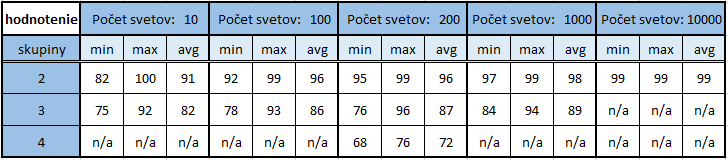
\includegraphics[scale=0.8]{img/ratingy.png}
\caption{Tabulka najlepších ohodnotení pri rôznych generovaniach herného sveta.}
\label{fig:ch51}
\end{figure}
\begin{figure}[H] 
\begin{center}
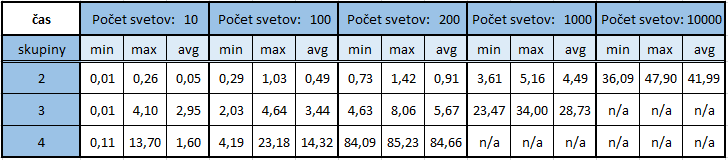
\includegraphics[scale=0.8]{img/casy.png}
\caption{Časy trvania rôznych generovaní herného sveta.}
\label{fig:ch52}
\end{center}
\end{figure}
Vygenerované svety následne slúžia ako množina z ktorej vyberieme svet s najlepšie ohodnotením príbehom. Na ľavej strane tabuľky máme zobrazené koľko skupín lokácii sme použili pri generovaní a zbytok tabuľky je rozdelený na časti v ktorých opisujeme hodnoty, ktoré sa vyskytli pri generovaní rôznych množstiev svetov naraz.\par
Z týchto hodnôt sme museli vydedukovať, koľko svetov sa nám oplatí generovať pred začiatkom hry, tak aby používateľ nečakal príliš dlho ale zároveň aby sa mu dostal obstojný príbeh. Vidíme, že pri dvoch skupinách lokácii nám stačí generovať sto svetov, pretože vyšším počtom už veľa na ohodnotení príbehu nezískame.\par
Ďaľší faktor, ktorý sme museli zohľadniť pri rozhodovaní je spolahlivosť. Čím viac svetov vygenerujeme tým je väčšia šanca, že vôbec nájdeme nejaký vygenerovaný svet, ktorý sa dá prejsť. Toto zohralo úlohu pri rozhodovaní sa pri troch skupinách, kde medzi generovaním sto alebo dvesto svetov nieje až taký rozdiel v štatistikách, ktoré sa týkajú ohodnotení vygenerovaných svetov ale ak vygenerujeme dvesto svetov tak máme v podstate dvojnásobne vyššiu pravdepodobnosť, že vygenerujeme hrateľný príbeh. Používateľ si síce o trochu viac počká ale šanca, že sa nevygeneruje hrateľný svet sa dvojnásobne zníži.\par
Pri štyroch skupinách lokácii sa veľmi neodporúča generovať herné svety, pretože generovanie je buď priveľmi nespolahlivé (malé množstvá generovaných svetov) alebo je nedostatočne rýchle aby bolo použiteľné. Vidíme, že pri nízkych počtoch vygenerovaných svetov sú hodnoty v tabuľke ohľadom hodnotenia prázdne a to preto, že sa pri týchto generovaniach nepodarilo vygenerovať nejaký hrateľný svet.\par
Čo sa časov týka, tak vidíme, že pri štyroch skupinách je generovanie dosť nepredvídateľné. Ak sa vygenerujú svety v ktorých plánovanie zistí celkom skoro, že svet nie je hrateľný tak sa generovanie skončí rýchlo. Komplikovanejšie svety však trvajú zase priveľmi dlho. Toto môžeme sledovať v tabuľke pri generovaní desiatich svetov, kde najkratšie trvalo 0,11 sekundy ale najdlhšie generovanie trvalo až 13,70 sekúnd. Pri generovaní sto svetov je čas uvedený v tabuľke za ktorý sa nepodarilo vygenerovať ani jeden hrateľný svet pretože pri tomto počte je toto generovanie ešte stále nespolahlivé. Pri dvesto svetoch generovanie začína byť ako tak spolahlivé ale čas generovania je neúnosný. Vyššie počty generovaných svetov sme ani neskúšali, pretože čas za ktorý by generovanie skončilo je nepriateľný na používanie aplikácie. To platí aj pri troch skupinách a desaťtisíc svetoch.\par
V tabuľke časov tiež môžeme vidieť, že zvýšením počtu skupín lokácii sa rapídne zvyšuje čas, ktorý je potrebný na generovanie takýchto svetov. Čas, ktorý tu narastá je čas plánovania príbehu. Ako môžeme vidieť na obrázku 5.3, tak dĺžky príbehov sa zvyšujú so zvýšeným počtom skupín lokácii.
\begin{figure}[H] 
\begin{center}
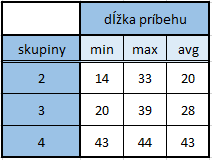
\includegraphics[scale=1.0]{img/dlzky.png}
\caption{Dĺžky príbehov pri rôžnych veľkostiach skupín lokácii.}
\label{fig:ch53}
\end{center}
\end{figure}
Toto je dôvodom zvyšujúceho sa času na generovanie herných svetov, keďže plánovanie príbehu je jeho súčasťou. A* vyhľadávanie má časovú zložitosť závislú od hĺbky vnorenia, ktorá je exponentom v tomto vzťahu, takže je zrejmé, že čas plánovania bude rásť tak rapídne ako nám ukazuje naša štatistika.\par
Dĺžka naplánovaného príbehu súvisí tiež aj s ohodnocovaním príbehu. Čím je príbeh dlhší, tým sa zvyšuje šanca na vyskytnutie sa niektorej z neželaných situácii v príbehu, ktoré my sledujeme a podľa ktorých príbeh hodnotíme. Túto skutočnosť môžeme tiež sledovať v tabuľke ohodnotení 5.1, kde vidieť, že čím viac skupín lokácii pri generovaní máme tým je priemerné ohodnotenie príbehu menšie.
\section{Výsledný príbeh}
Naša aplikácia generuje príbehy o princovi, ktorý sa snaží zachrániť princeznú, ktorú uniesli banditi nikto nevie kam. Títo banditi požadujú výkupné za unesenú princeznú. Princ bude musieť prekonávať prekážky na ceste za princeznou ako napríklad riešiť rôzne hádanky alebo bojovať s príšerami. Navyše musí nejako získať mince na výkupné za princeznú.\par
Najprv si ukážeme jeden z horšie ohodnotených príbehov podľa našej hypotézi. Môžeme ho vidieť na obrázku 5.4 a popíšeme si prečo ho tak naša aplikácia ohodnotila.
\begin{figure}[H] 
\begin{center}
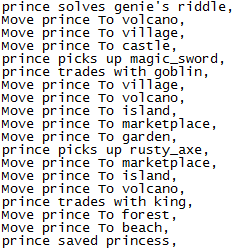
\includegraphics[scale=1.0]{img/zly_pribeh.png}
\caption{Ukážka menej zaujímavého príbehu.}
\label{fig:ch54}
\end{center}
\end{figure}
Hneď prvá akcia príbehu je jednou z chýb prečo má tento príbeh zlé ohodnotenie. Podľa našeho prístupu by hráč nemal hned riešiť úlohy, ktoré posúvajú príbeh a táto akcia je jednou z nich. Hráč by sa mal na začiatku trochu spoznať s prostredím a objavovať.\par
Druhou chybou je zbytočná dĺžka príbehu. Príbeh má zbytočne veľa akcii a veľa krát sa v ňom opakuje akcia Move. Viac ako polovicu príbehu zaberá len premiestňovanie sa, čo je podľa nás nezaujímavé a aj kvôli tomuto má príbeh znížené hodnotenie.\par
Posledná chyba v tomto príbehu sa týka akcii PickUp a Trade, ktoré sú v príbehu hneď po sebe, čo znamená že obchodník aj vec, ktorú tento obchodník chce kúpiť sa nachádzajú na tej istej lokácii. Toto je nežiadúca situácia, pretože obchodník týmto stráca význam, keďže hráč danú vec nemusí hľadať.\par
Ďalej si ukážeme príbeh, ktorý naša aplikácia ohodnotila vyskoým hodnotením a popíšeme, prečo si myslíme, že je hodný vysokého hodnotenia. Tento príbeh je zobrazený na obrázku 5.5.
\begin{figure}[H] 
\begin{center}
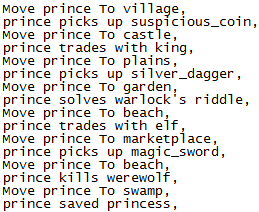
\includegraphics[scale=1.0]{img/dobry_pribeh.png}
\caption{Ukážka viac zaujímavého príbehu.}
\label{fig:ch55}
\end{center}
\end{figure}
V tomto príklade môžeme vidieť, že sa príbeh nezačína akciou posúvajúcou príbeh. Toto je známkou dobrého úvodu hráča do deja a zoznámenia sa s príbehom a svetom.\par
Ďaľej môžme pozorovať, že príbeh nie je zbytočne natiahnutý opakujúcimi sa akciami, čo znamená že hráč sa neunudí v zdĺhavých častiach príbehu. Akcie sa v príbehu striedajú a teda príbeh necháva hráča objavovať svet a hľadať v ňom zaujímavé veci ale zároveň aj ponúka posun príbehu k cieľu. Toto striedanie akcii navyše zaručuje, že žiadna zápletka nie je zbytočná, ako sme mohli vidieť v príbehu z obrázku 5.4, kde jeden z obchodníkov bol nezaujímavý a vlastne zbytočný.\par